\chapter{Lorentztransformatie van impuls en energie}
\vspace{-1cm}\begin{flushright}
{\it `Experts are just trained dogs'}\\ A. Einstein
\end{flushright}

\section{Viervectoren}
Natuurkundige verschijnselen spelen zich dus af in een
vierdimensionale wereld\footnote{Moderne en uit theoretisch oogpunt
aantrekkelijke natuurkundige theori\"{e}n (`string theories') hebben
aan vier dimensies niet genoeg.}: drie ruimte dimensies en een tijd
dimensie die nauw verweven zijn.  Een `plaats' in deze
vierdimensionale wereld wordt dus aangegeven door vier getallen, een
vierdimensionale vector: $(x, y, z, ct)$.  Deze vector transformeert
onder Lorentztransformaties volgens de formules die we zojuist
gevonden hebben.  Zo'n vector noemen we een viervector.  De {\it norm}
(`grootte' in deze speciale ruimte) van de viervector is gelijk aan
$x^{2} + y^{2} + z^{2} - c^{2}t^{2}$ en is \underline{invariant} onder
Lorentztransformaties. De waarde van de norm is dus gelijk voor elk
inertiaalsysteem; dit geldt niet voor de afzonderlijke
co\"ordinaten. Vergelijk dit met de lengte van een vector in een
drie-dimensionaal co\"ordinatenstelsel; deze lengte is invariant in de
drie-dimensionale wereld.  Later zullen we zien dat impuls en energie
ook een viervector vormen, en dat dus ook de norm van deze vier-vector
invariant is.


\section{Impuls}
Een `object', denk voor het gemak aan een puntmassa, met massa $m$ en snelheid
$\vec{v}$ heeft, per definitie, een impuls
\begin{displaymath}
\vec{p} = m\vec{v}
\end{displaymath}
Een belangrijke reden om de grootheid impuls in de mechanica in te voeren
is het feit dat impuls een \underline{behouden grootheid} is.
Dit betekent dat een mechanisch systeem dat aan zijn lot overgelaten wordt
(een enkel deeltje; twee botsende deeltjes; het heelal) of iets
preciezer geformuleerd: een gesloten\footnote{D.w.z. niet wisselwerkend met de omgeving.}
mechanisch systeem steeds dezelfde impuls heeft.

% \begin{figure}[h]
% \begin{center}
% \mbox{\epsfxsize=10cm\epsffile{syllabus.pictures/botsing1.eps}}
% \caption{Botsende deeltjes}
% \label{f:impuls1}
% \end{center}
% \end{figure}

\begin{figure}[ht]
\centering
\includegraphics[width=.7\textwidth]{syllabus.pictures/botsing1}
\caption{Botsende deeltjes}
\label{f:impuls1}
\end{figure}


% \begin{figure}[h]
% \begin{center}
% \mbox{\epsfxsize=10cm\epsffile{syllabus.pictures/botsing2.eps}}
% \caption{Botsende deeltjes}
% \label{f:impuls2}
% \end{center}
% \end{figure}

\begin{figure}[ht]
\centering
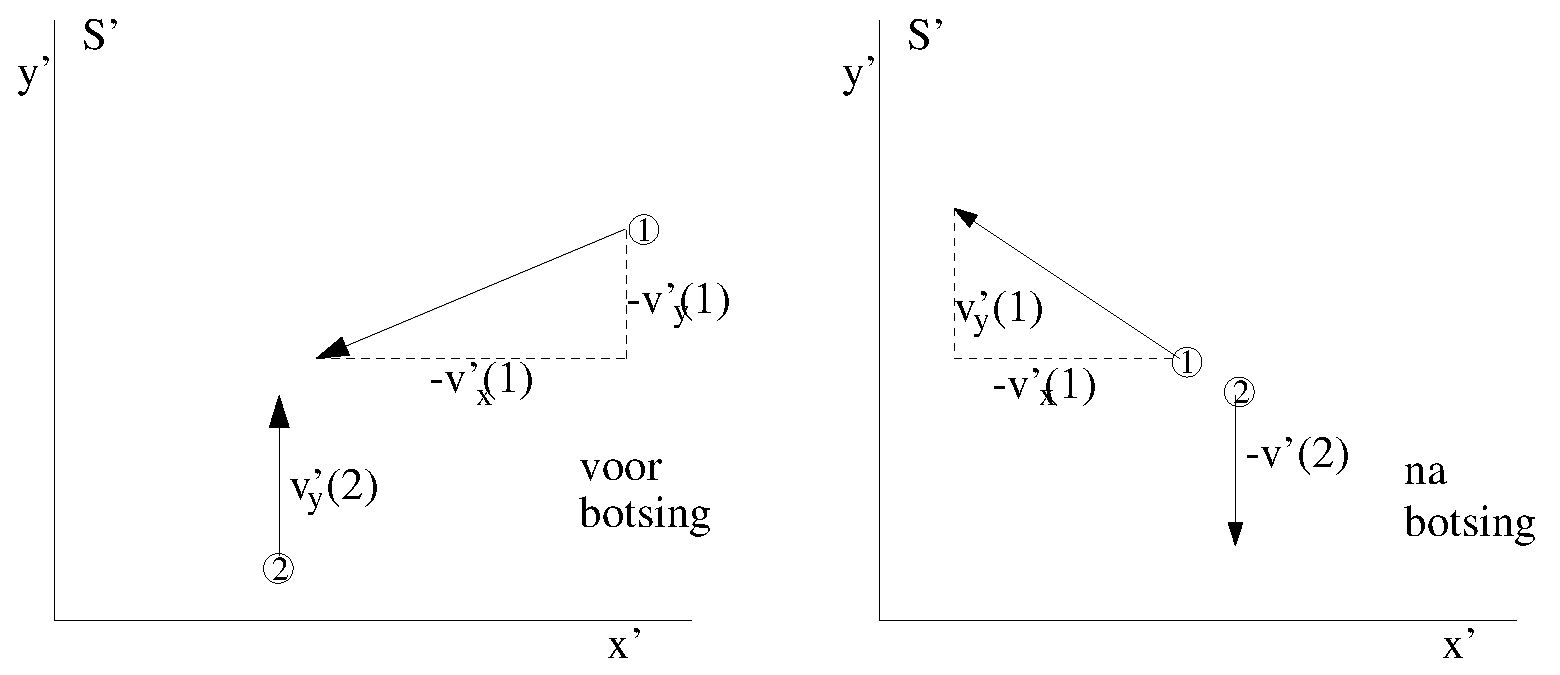
\includegraphics[width=.7\textwidth]{syllabus.pictures/botsing2}
\caption{Botsende deeltjes}
\label{f:impuls2}
\end{figure}


We bekijken als voorbeeld twee elastisch botsende puntmassa's ieder met
massa $M$ zoals aangegeven in figuur \ref{f:impuls1}. 

In systeem $S'$ dat met puntmassa $2$ mee beweegt in de $x$-richting
ziet de situatie er uit als in figuur \ref{f:impuls2}

In systeem $S$ betekent impulsbehoud;
\begin{eqnarray*}
\{p_{x}(1) + p_{x}(2)\}_{voor} & = & \{p_{x}(1) + p_{x}(2)\}_{na} \\
\{p_{y}(1) + p_{y}(2)\}_{voor} & = & \{p_{y}(1) + p_{y}(2)\}_{na}
\end{eqnarray*}
(We hebben ons voorbeeld z\'{o} gekozen dat de totale impuls in zowel 
de $x$-richting als de $y$-richting gelijk is aan 0.)

Uit impulsbehoud volgt dat de impulsverandering van puntmassa $1$ gelijk is in
grootte en tegengesteld in richting aan de impulsverandering van puntmassa
$2$:
\begin{eqnarray*}
p_{x}(1)_{voor} - p_{x}(1)_{na} & = & 
-(p_{x}(2)_{voor} - p_{x}(2)_{na})  \\
p_{y}(1)_{voor} - p_{y}(1)_{na} & = & 
-(p_{y}(2)_{voor} - p_{y}(2)_{na})
\end{eqnarray*}
In $S'$ moet impulsbehoud ook gelden (2de postulaat).
In de $x$-richting geldt dit zonder meer: zowel de impulsverandering van $1$ 
als $2$ is nul.

In de $y$-richting lijken we echter op een probleem te stuiten.
M.b.v. de transformatieformules voor de snelheid vinden we:
\begin{equation}
\label{v:impuls1}
v'_{y}(1) = \frac{-v_{y}}{1 + \frac{v^{2}_{x}}{c^{2}}} \sqrt{1 - \frac{v^{2}_{x}}{c^{2}}}
\end{equation}
\begin{equation}
\label{v:impuls2}
v'_{y}(2) = \frac{v_{y}}{1 - \frac{v^{2}_{x}}{c^{2}}} \sqrt{1 - \frac{v^{2}_{x}}{c^{2}}}
\end{equation}
Indien we de impuls weer defini\"{e}ren als $Mv'_{y}(1)$ resp. $Mv'_{y}(2)$
dan zien we dat de impulsverandering van puntmassa $1$, $2Mv'_{y}(1)$, niet 
gelijk is in grootte aan die van puntmassa $2$, $2Mv'_{y}(2)$.
M.a.w. impulsbehoud impliceert dat we onze definitie van impuls moeten herzien!

We zien dat de Lorentztransformatie in de $x$-richting de \underline{snelheid}
in de $y$-richting doet veranderen en dat is de bron van onze `moeilijkheden'.
We proberen nu een definitie van impuls te vinden z\'{o} dat een transformatie
in de $x$-richting de impuls in de $y$-richting onveranderd laat.
Terugkerend naar ons voorbeeld willen we dus:
\begin{displaymath}
p'_{y}(2) = p_{y}(2)
\end{displaymath}
We schrijven formeel (het is maar een poging):
\begin{displaymath}
M'_{2}v'_{y}(2) = M_{2}v_{y}
\end{displaymath}
en invullen van \ref{v:impuls2} levert nu:
\begin{equation}
\label{v:impuls3}
M'_{2} = M_{2} \sqrt{1 - \frac{v^{2}_{x}}{c^{2}} }
\end{equation}
Een analoge redenering voor puntmassa $1$ levert:
\begin{equation}
\label{v:impuls4}
M'_{1} =  \frac{1 + \frac{v^{2}_{x}}{c^{2}}} {\sqrt{1 - \frac{v^{2}_{x}}{c^{2}}}} M_{1}
\end{equation}
We zien dus dat een correcte definitie van impuls de volgende vorm zal hebben:
\begin{displaymath}
p = f_{s}Mv
\end{displaymath}
waar $f_{s}$ een kinematische factor is die samenhangt met het referentiesysteem waarin we kijken, $M$ de massa is en $v$ de snelheid.

Hierdoor ge\"{i}nspireerd schrijven we nu:
\begin{eqnarray*}
M'_{2} & = & aM \\
M_{2} & = & bM \\
M'_{1} & = & qM \\
M_{1} & = & rM
\end{eqnarray*}
Omdat de puntmassa's $1$ en $2$ t.o.v. $S$ in feite dezelfde beweging uitvoeren
(`verwisselbaar zijn') zal moeten gelden $b = r$.\\
Maken we nu gebruik van \ref{v:impuls3} en \ref{v:impuls4}
dan zien we:
\begin{eqnarray*}
a & = & b\sqrt{1 - \frac{v^{2}_{x}}{c^{2}}} \\
q & = & b\frac{1 + \frac{v^{2}_x}{c^{2}}}{\sqrt{1 - \frac{v^{2}_{x}}{c^{2}}}}
\end{eqnarray*}
Dit zijn twee vergelijkingen met drie onbekenden en zonder extra inspiratie
kunnen we niet verder komen dan:
\begin{eqnarray*}
M'_{2} & = & b \sqrt{1 - \frac{v^{2}_{x}}{c^{2}}} M \\
M_{2} & = & bM \\
M'_{1} & = & b\frac{1 + \frac{v^{2}_x} {c^{2}} }
{\sqrt{1 - \frac{v^{2}_{x}} {c^{2}} } } M \\
M_{1} & = & bM
\end{eqnarray*}
We zouden de massa nu kunnen herdefini\"{e}ren als ${\cal M} = bM$ maar dat is 
onbevredigend want dan zou $\cal M$ de massa zijn zoals die geldt in
systeem $S$ en we willen de massa defini\"{e}ren als een eigenschap
van een object (deeltje),
onafhankelijk van de bewegingstoestand.

Zonder een meer volledige beschouwing, waarin we ook energie betrekken, 
zitten we vast.
We gaan daarom een redelijke gok maken van $b$ en laten zien dat deze gok 
in overeenstemming is met een consistente definitie van impuls en energie. 

Bekijk nog eens:
\begin{displaymath}
M_{1} = M_{2} = bM
\end{displaymath}
$b$ hangt af van $v$ (niet van de richting van $v$) en we vermoeden
dat $b \rightarrow 1$ als $v \rightarrow 0$, of liever
$\frac{v}{c} \rightarrow 0$.
Hier is onze gok (weliswaar met voorkennis....):
\begin{displaymath}
b = \frac{1}{\sqrt{1 - \frac{v^{2}_{x} + v^{2}_{y}}{c^{2}}}}
\end{displaymath}
Dit leidt tot de definitie van relativistische impuls:
\begin{equation}
\label{v:impuls5}
\vec{p} = \frac{M\vec{v}}{\sqrt{1 - \frac{v^{2}} {c^{2}} } }
\end{equation}
of
\begin{displaymath}
\vec{p}~=~\gamma M \vec{v}
\end{displaymath}
M.a.w. een massa $M$ met snelheid $\vec{v} = (v_{x}, v_{y}, v_{z})$,
dus $v^{2} = v^{2}_{x} + v^{2}_{y} + v^{2}_{z}$, heeft een impuls als 
in formule \ref{v:impuls5} aangegeven.
Als $\frac{v}{c} \rightarrow 0$ is $\vec{p} = M \vec{v}$.
Voor de grootte van de impuls geldt dus:
\begin{displaymath}
p = \frac{Mv}{\sqrt{1 - \frac{v^{2}}{c^{2}} } }
\end{displaymath}
of
\begin{equation}
\label{v:impuls}
p = M\beta\gamma c
\end{equation}

We kunnen ons nu afvragen hoe impuls transformeert onder een
Lorentztransformatie. Een Lorentztransformatie is een transformatie
in een vier-dimensionale ruimte (plaats-tijd). Impuls is echter een
vector in een drie-dimensionale ruimte, we moeten dus een vierde
component toevoegen om een Lorentztransformatie te kunnen toepassen.
Hoe deze vierde component er precies uitziet moeten we nader bepalen.

Onze afleiding van de correcte formule voor relativistische impuls
heeft ons geleerd dat de impulscomponenten loodrecht op de 
transformatierichting niet veranderen onder de transformatie.
Dit doet ons denken aan de componenten van de plaatsvector loodrecht
op de transformatierichting: die veranderen ook niet.
Construeer nu de volgende vierdimensionale vector: $(\vec{p},A)$ en
probeer een $A$ te vinden zodat dit een echte viervector is, d.w.z.
een vector die transformeert onder Lorentztransformaties zoals 
de ruimte-tijd viervector $(\vec{r},ct)$.

Beschouw massa $M$ die beweegt met snelheid $v_x$ in de $x$-richting
t.o.v. inertiaalstelsel $S$. T.o.v. inertiaalstelsel $S^\prime$ dat
met snelheid $v_x$ beweegt in de $x$-richting t.o.v. inertiaalstelsel $S$
staat de massa $M$ dus stil.

Indien we op $(\vec{p},A)$ de Lorentztransformatie toepassen zoals die
geldt voor $(\vec{r},ct)$, dan vinden we:
\begin{eqnarray*}
p_x^\prime & = & \gamma p_x~-~\beta \gamma A \\
A^\prime & = & \gamma A~-~\beta \gamma p_x 
\end{eqnarray*}

In de bovengeschetste situatie is $p_x^\prime=0$ en vinden we
$A=p_x/\beta$. Echter: $p_x=M\gamma \beta c$ (zelfde $\gamma$ en
$\beta$ als in de Lorentztransformatie die we beschouwen, ga dit
na!) en vinden we $A=\gamma Mc$.

Verder vinden we $A^\prime=Mc$ (ga na).

Een eigenschap van viervectoren is dat hun norm invariant is:
d.w.z. dat de norm van een viervector gelijk is aan de norm
van de getransformeerde viervector. Dus we moeten verifieren of:
\begin{displaymath}
p_x^{\prime 2}+p_y^{\prime 2}+p_z^{\prime 2}-A^{\prime 2}=p_x^{2}+p_y^{2}+p_z^{2}-A^{2}
\end{displaymath}

Het is heel gemakkelijk na te gaan dat dit inderdaad zo is en dat
$p^2-A^2=p^{\prime 2}-A^{\prime 2}=-M^2c^2$.

Wat is de betekenis van $A=\gamma M c = Mc/\sqrt{1-v^2/c^2}$?

Bekijk de niet-relativistische limiet $v/c \ll 1$, dan geldt de
benadering $1/\sqrt{1-v^2/c^2}\simeq 1+v^2/2c^2$ en vinden we
$A~=~ Mc~+~Mv^2/2c^2$ of $Ac~=~Mc^2~+~Mv^2/2$. $Ac$ is dus
de bekende kinetische energie plus een constante. Met andere
woorden de vierde component van de viervector die we hier beschouwen
is de energie (gedeeld door $c$). We hebben nu de impuls-energie
viervector gevonden: $(\vec{p},E/c)$ of $(\vec{p}c,E)$ met als
norm:
\begin{displaymath}
E^2~-~p^2c^2~=~M^2c^4
\end{displaymath}
Deze formule, samen met de relatie 
\begin{displaymath}
p=\frac{\beta E}{c}
\end{displaymath}
of, beter,
\begin{displaymath}
\vec{p}=\frac{\vec{v} E}{c^2}
\end{displaymath}

vormen samen de fundamentele relativistische relaties voor een vrij
bewegend deeltje.

\section{Energie}
Net als impuls ($p_{x}, p_{y}, p_{z}$) blijkt het mogelijk een andere
fundamentele, behouden grootheid te defini\"{e}ren, de energie.
Zo is de energie van een vrij bewegende puntmassa $M$ en snelheid $v$,
in de niet-relativistische mechanica gelijk aan $\frac{1}{2}Mv^{2}$, ook
wel de kinetische energie genoemd.\\
Indien we ook energiebehoud willen laten gelden onafhankelijk
van het referentiestelsel waarin we kijken, dan moet ook
de definitie van energie herzien worden en natuurlijk ook weer z\'{o},
dat in de limiet $\frac{v}{c} \rightarrow 0$ de formule
$\frac{1}{2}Mv^{2}$ teruggevonden wordt.
We zullen hier geen poging doen de goede formule `af te leiden'
maar, omgekeerd, de goede formule aan de litteratuur ontlenen en aantonen
dat ze werkt\footnote{De oorspronkelijke afleiding van Einstein maakt gebruik van 
elementaire maar in dit stadium van het curriculum nog niet behandelde
theorie van elektrodynamica.}.

We schrijven:
\begin{displaymath}
E = \frac{Mc^{2}} {\sqrt{1 - \frac{v^{2}} {c^{2}} }}
\end{displaymath}
of
\begin{equation}
\label{v:energie}
E = M\gamma c^{2}
\end{equation}
Indien $\frac{v}{c} \ll 1$ dan geldt:
\begin{displaymath}
\frac{1} {\sqrt{1 - \frac{v^{2}} {c^{2}}}}
\cong 1 + \frac{v^{2}} {2c^{2}}
\end{displaymath}

en in de niet-relativistische limiet vinden we dus:

\begin{displaymath}
E = Mc^{2} + \frac{1}{2}Mv^{2}
\end{displaymath}

Dit is precies de bekende kinematische energie plus een constante,
$Mc^{2}$ (energiebehoud wordt door dergelijke constanten uiteraard netjes 
in tact gelaten).

\section{De impuls-energie viervector}
Het is nu gemakkelijk om na te gaan hoe impuls en energie transformeren
onder een Lorentztransformatie.\\
Een puntmassa heeft een impuls $\vec{p}$ (snelheid $\vec{v}$) en
energie $E$ in $S$.\\
$S'$ beweegt met snelheid $V$ (het symbool $v$ is al vergeven aan de 
snelheid van de puntmassa t.o.v. $S$) in de
positieve $x$-richting t.o.v. $S$.
T.o.v. $S'$ zijn impuls $\vec{p'}$ en energie $E'$ dan:
\begin{eqnarray*}
p'_{x} & = & \gamma(p_{x} - \beta \frac{E}{c}) \\
p'_{y} & = & p_{y} \\
p'_{z} & = & p_{z} \\
\frac{E'}{c} & = & \gamma (\frac{E}{c} - \beta p_{x})
\end{eqnarray*}
waar $\gamma = \frac{1}{\sqrt{1-V^2/c^2}} = \frac{1}{\sqrt{1-\beta ^{2}}}$\\
Merk op, dat dit precies dezelfde transformatie is als die van $(\vec{r}, ct)$
met de rol van $\vec{r}$ overgenomen door $\vec{p}$
en die van $ct$ door $E/c$.\\
Net zoals 
$c^{2}t^{2} - x^{2} - y^{2} -z^{2} = c^{2}t'^{2} - x'^{2} - y'^{2} -z'^{2}$,
d.w.z.  $c^{2}t^{2} - x^{2} - y^{2} -z^{2}$
invariant is onder Lorentztransformaties, geldt dit nu ook voor
\begin{displaymath}
\frac{E^{2}}{c^{2}} - p^{2}_{x} - p^{2}_{y} - p^{2}_{z} = \frac{E'^{2}}{c^{2}} - p'^{2}_{x} - p'^{2}_{y} - p'^{2}_{z}
\end{displaymath}
Uitrekenen levert:
\begin{displaymath}
E^{2} - p^{2}_{x}c^{2} - p^{2}_{y}c^{2} - p^{2}_{z}c^{2} = M^{2}c^{4}
\end{displaymath}
of
\begin{displaymath}
Mc^{2} = \sqrt{E^{2} - \vec{p}^{2}c^{2}}
\end{displaymath}

\section{Energie en massa}
Voor een deeltje in rust geldt dus de beroemde formule
\begin{displaymath}
E = Mc^{2}
\end{displaymath}
Een spectaculaire consequentie van deze 'equivalentie van massa en energie'
is dat massa, in principe, in energie kan worden omgezet.

\section{Massaloze deeltjes}
We zien dat de relativiteitstheorie massaloze deeltjes toelaat:
\begin{displaymath}
E = pc
\end{displaymath}
leidt tot
\begin{displaymath}
M = 0
\end{displaymath}
Aangezien uit formules \ref{v:impuls} en \ref{v:energie} volgt dat
\begin{displaymath}
p = \frac{E}{c} \beta 
\end{displaymath}
(ga na) geldt voor massaloze deeltjes dus:
\begin{displaymath}
p = \frac{pc}{c} \beta = p \beta
\end{displaymath}
Hieruit volgt dat $\beta = 1$, dus $v = c$.
M.a.w. massaloze deeltjes bewegen met de lichtsnelheid.


%%% Local Variables: 
%%% mode: latex
%%% TeX-master: "Impuls"
%%% End: 
